% move all configuration stuff into one file so we can focus on the content
\documentclass[aspectratio=169,hyperref={pdfpagelabels=false,colorlinks=true,linkcolor=white,urlcolor=blue},t]{beamer}

%%%%%%%%%%%%%%%%%%%%%%%%%%%%%%%%%%%%%%%%%%%%%%%%%%%%%%%%%%%%%%%%%%%%%%%%%%%%%%%%%%
%%%%%%%%%%%%%%%%%%%%%%%%%%%%%%%%%%%%%%%%%%%%%%%%%%%%%%%%%%%%%%%%%%%%%%%%%%%%%%%%%%
% packages
\usepackage{pict2e}
\usepackage{epic}
\usepackage{amsmath,amsfonts,amssymb}
\usepackage{units}
\usepackage{fancybox}
\usepackage[absolute,overlay]{textpos} 
\usepackage{media9} % avi2flv: "C:\Program Files\ffmpeg\bin\ffmpeg.exe" -i TuneFreqFilterbank.avi -b 600k -s 441x324 -r 15 -acodec copy TuneFreqFilterbank.flv
\usepackage{animate}
\usepackage{gensymb}
\usepackage{multirow}
\usepackage{silence}
\usepackage[backend=bibtex,style=ieee]{biblatex}
\AtEveryCitekey{\iffootnote{\tiny}{}}
\addbibresource{references}

%%%%%%%%%%%%%%%%%%%%%%%%%%%%%%%%%%%%%%%%%%%%%%%%%%%%%%%%%%%%%%%%%%%%%%%%%%%%%%%%%%
%%%%%%%%%%%%%%%%%%%%%%%%%%%%%%%%%%%%%%%%%%%%%%%%%%%%%%%%%%%%%%%%%%%%%%%%%%%%%%%%%%
% relative paths
\graphicspath{{graph/}}


%%%%%%%%%%%%%%%%%%%%%%%%%%%%%%%%%%%%%%%%%%%%%%%%%%%%%%%%%%%%%%%%%%%%%%%%%%%%%%%%%%
%%%%%%%%%%%%%%%%%%%%%%%%%%%%%%%%%%%%%%%%%%%%%%%%%%%%%%%%%%%%%%%%%%%%%%%%%%%%%%%%%%
% units
\setlength{\unitlength}{1mm}

%%%%%%%%%%%%%%%%%%%%%%%%%%%%%%%%%%%%%%%%%%%%%%%%%%%%%%%%%%%%%%%%%%%%%%%%%%%%%%%%%%
%%%%%%%%%%%%%%%%%%%%%%%%%%%%%%%%%%%%%%%%%%%%%%%%%%%%%%%%%%%%%%%%%%%%%%%%%%%%%%%%%%
% theme & layout
\usetheme{Frankfurt}
\beamertemplatenavigationsymbolsempty
%\setbeamertemplate{frametitle}[smoothbars theme]
\setbeamertemplate{frametitle}
{
    \begin{beamercolorbox}[ht=1.8em,wd=\paperwidth]{frametitle}
        \vspace{-.1em}%
        \hspace{.2em}{\strut\insertframetitle\strut}
        
        \hspace{.2em}\small\strut\insertframesubtitle\strut
        %\hfill
        %
\includegraphics[height=.8cm,keepaspectratio]{CenterMusicTechnology-solid-2lines-white-CoAtag}
        
    \end{beamercolorbox}
    \begin{textblock*}{100mm}(11.6cm,.7cm)
        \includegraphics[height=.8cm,keepaspectratio]{logo_GTCMT_black}
    \end{textblock*}
}

% set this to ensure bulletpoints without subsections
\usepackage{remreset}
\makeatletter
\@removefromreset{subsection}{section}
\makeatother
\setcounter{subsection}{1}

%---------------------------------------------------------------------------------
% appearance
\setbeamercolor{structure}{fg=gtgold}
\setbeamercovered{transparent} %invisible
\setbeamercolor{bibliography entry author}{fg=black}
\setbeamercolor*{bibliography entry title}{fg=black}
\setbeamercolor*{bibliography entry note}{fg=black}

%\usepackage{pgfpages}
%\setbeameroption{show notes}
%\setbeameroption{show notes on second screen=right}
%---------------------------------------------------------------------------------
% fontsize
\let\Tiny=\tiny

%%%%%%%%%%%%%%%%%%%%%%%%%%%%%%%%%%%%%%%%%%%%%%%%%%%%%%%%%%%%%%%%%%%%%%%%%%%%%%%%%%
%%%%%%%%%%%%%%%%%%%%%%%%%%%%%%%%%%%%%%%%%%%%%%%%%%%%%%%%%%%%%%%%%%%%%%%%%%%%%%%%%%
% warnings
\pdfsuppresswarningpagegroup=1
\WarningFilter{biblatex}{Patching footnotes failed}
\WarningFilter{latexfont}{Font shape}
\WarningFilter{latexfont}{Some font shapes}
\WarningFilter{gensymb}{Not defining}



\subtitle{Part 4.1: Instantaneous Features~---~Introduction}

%%%%%%%%%%%%%%%%%%%%%%%%%%%%%%%%%%%%%%%%%%%%%%%%%%%%%%%%%%%%%%%%%%%%%%%%%%%%
\begin{document}
    % generate title page
	

\begin{frame}
    \titlepage
    %\vspace{-5mm}
    \begin{flushright}
        \href{http://www.gtcmt.gatech.edu}{\includegraphics[height=.8cm,keepaspectratio]{logo_GTCMT_black}}
    \end{flushright}
\end{frame}


    \section[overview]{lecture overview}
        \begin{frame}{instantaneous features}{overview}
            \begin{itemize}
                \item   \textbf{text book}  
                    \begin{itemize}
                        \item   \href{http://ieeexplore.ieee.org/xpl/articleDetails.jsp?tp=&arnumber=6331120&}{\underline{\textit{Chapter 3: Instantaneous Features} (pp.~31--41)}}
                    \end{itemize}
                \bigskip
                \item<2->   \textbf{lecture content}
                    \begin{itemize}
                        \item<2->   feature extraction 
                        \item<3->   feature pre-processing
                        \item<4->   statistical features
                    \end{itemize}
            \end{itemize}
        \end{frame}

    \section[intro]{introduction}
        \begin{frame}{instantaneous features}{introduction}
            remember the flow chart of a general ACA system:
            \vspace{-2mm}
            \begin{figure}
                \begin{footnotesize}
				\begin{picture}(96,26)
					\setcounter{iXOffset}{0}
					\setcounter{iYOffset}{5}
					\setcounter{iXBlockSize}{28}
					\setcounter{iYBlockSize}{16}
					\setcounter{iYBlockSizeDiv2}{8}
					\setcounter{iDistance}{8}
	
					\addtocounter{iYOffset}{\value{iYBlockSizeDiv2}}
					\addtocounter{iYOffset}{-2}
	
					%\addtocounter{iXOffset}{-1}
					\put(\value{iXOffset}, \value{iYOffset})
						{\text{{\shortstack[c]{audio\\ signal}}}}
					\addtocounter{iXOffset}{1}
	
					\addtocounter{iYOffset}{2}
					\addtocounter{iXOffset}{\value{iDistance}}
	
					\put(\value{iXOffset}, \value{iYOffset})
						{\vector(1,0){\value{iDistance}}}
	
					\addtocounter{iXOffset}{\value{iDistance}}
					\addtocounter{iYOffset}{-\value{iYBlockSizeDiv2}}
					
					\put(\value{iXOffset}, \value{iYOffset})
						{\framebox(\value{iXBlockSize}, \value{iYBlockSize}) {\color{gtgold}{\shortstack[c]{feature\\ extraction}}}}
	
					\addtocounter{iXOffset}{\value{iXBlockSize}}
					\addtocounter{iYOffset}{\value{iYBlockSizeDiv2}}
	
					\put(\value{iXOffset}, \value{iYOffset})
						{\vector(1,0){\value{iDistance}}}
	
					\addtocounter{iXOffset}{\value{iDistance}}
					\addtocounter{iYOffset}{-\value{iYBlockSizeDiv2}}
	
					\put(\value{iXOffset}, \value{iYOffset})
						{\framebox(\value{iXBlockSize}, \value{iYBlockSize}) {\shortstack[c]{decision,\\ interpretation,\\ classification,\\ inference}}}
	
					\addtocounter{iXOffset}{\value{iXBlockSize}}
					\addtocounter{iYOffset}{\value{iYBlockSizeDiv2}}
	
					\put(\value{iXOffset}, \value{iYOffset})
						{\vector(1,0){\value{iDistance}}}
	
					\addtocounter{iXOffset}{\value{iDistance}}
					\addtocounter{iYOffset}{-2}
	
					\addtocounter{iXOffset}{1}
					\put(\value{iXOffset}, \value{iYOffset})
						{\text{{\shortstack[c]{meta\\ data}}}}
					
				\end{picture}
\end{footnotesize}

            \end{figure}
            
            \vspace{-2mm}
            \pause
            \textbf{feature}:
            \begin{itemize}
                \item<2->   \textit{terminology}: 
                    \begin{itemize}
                        \item   audio descriptor
                        \item   instantaneous/short-term/\color<3->{gtgold}{low-level feature}
                    \end{itemize}
                \item<3->   \textit{characteristics}:
                    \begin{itemize}
                        \item	not necessarily musically, perceptually, or semantically meaningful
                        \item	usually one feature per block of data
                    \end{itemize}
            \end{itemize}
        \end{frame}
        \begin{frame}{instantaneous features}{feature}
            \only<1-5>{
            \toremember{a feature \ldots}
            
            \begin{itemize}
                \item   has to be task-specific,
                \item<2->   is often chosen from a set of established features, but
                \item<3->   can be invented/customized, and
                \item<4->   can also be derived from other data (tags, etc.), or
                \item<5->   from other features.
            \end{itemize}
            }
            \only<6>{
                \begin{columns}
                \column{.7\linewidth}
                \begin{figure}
                    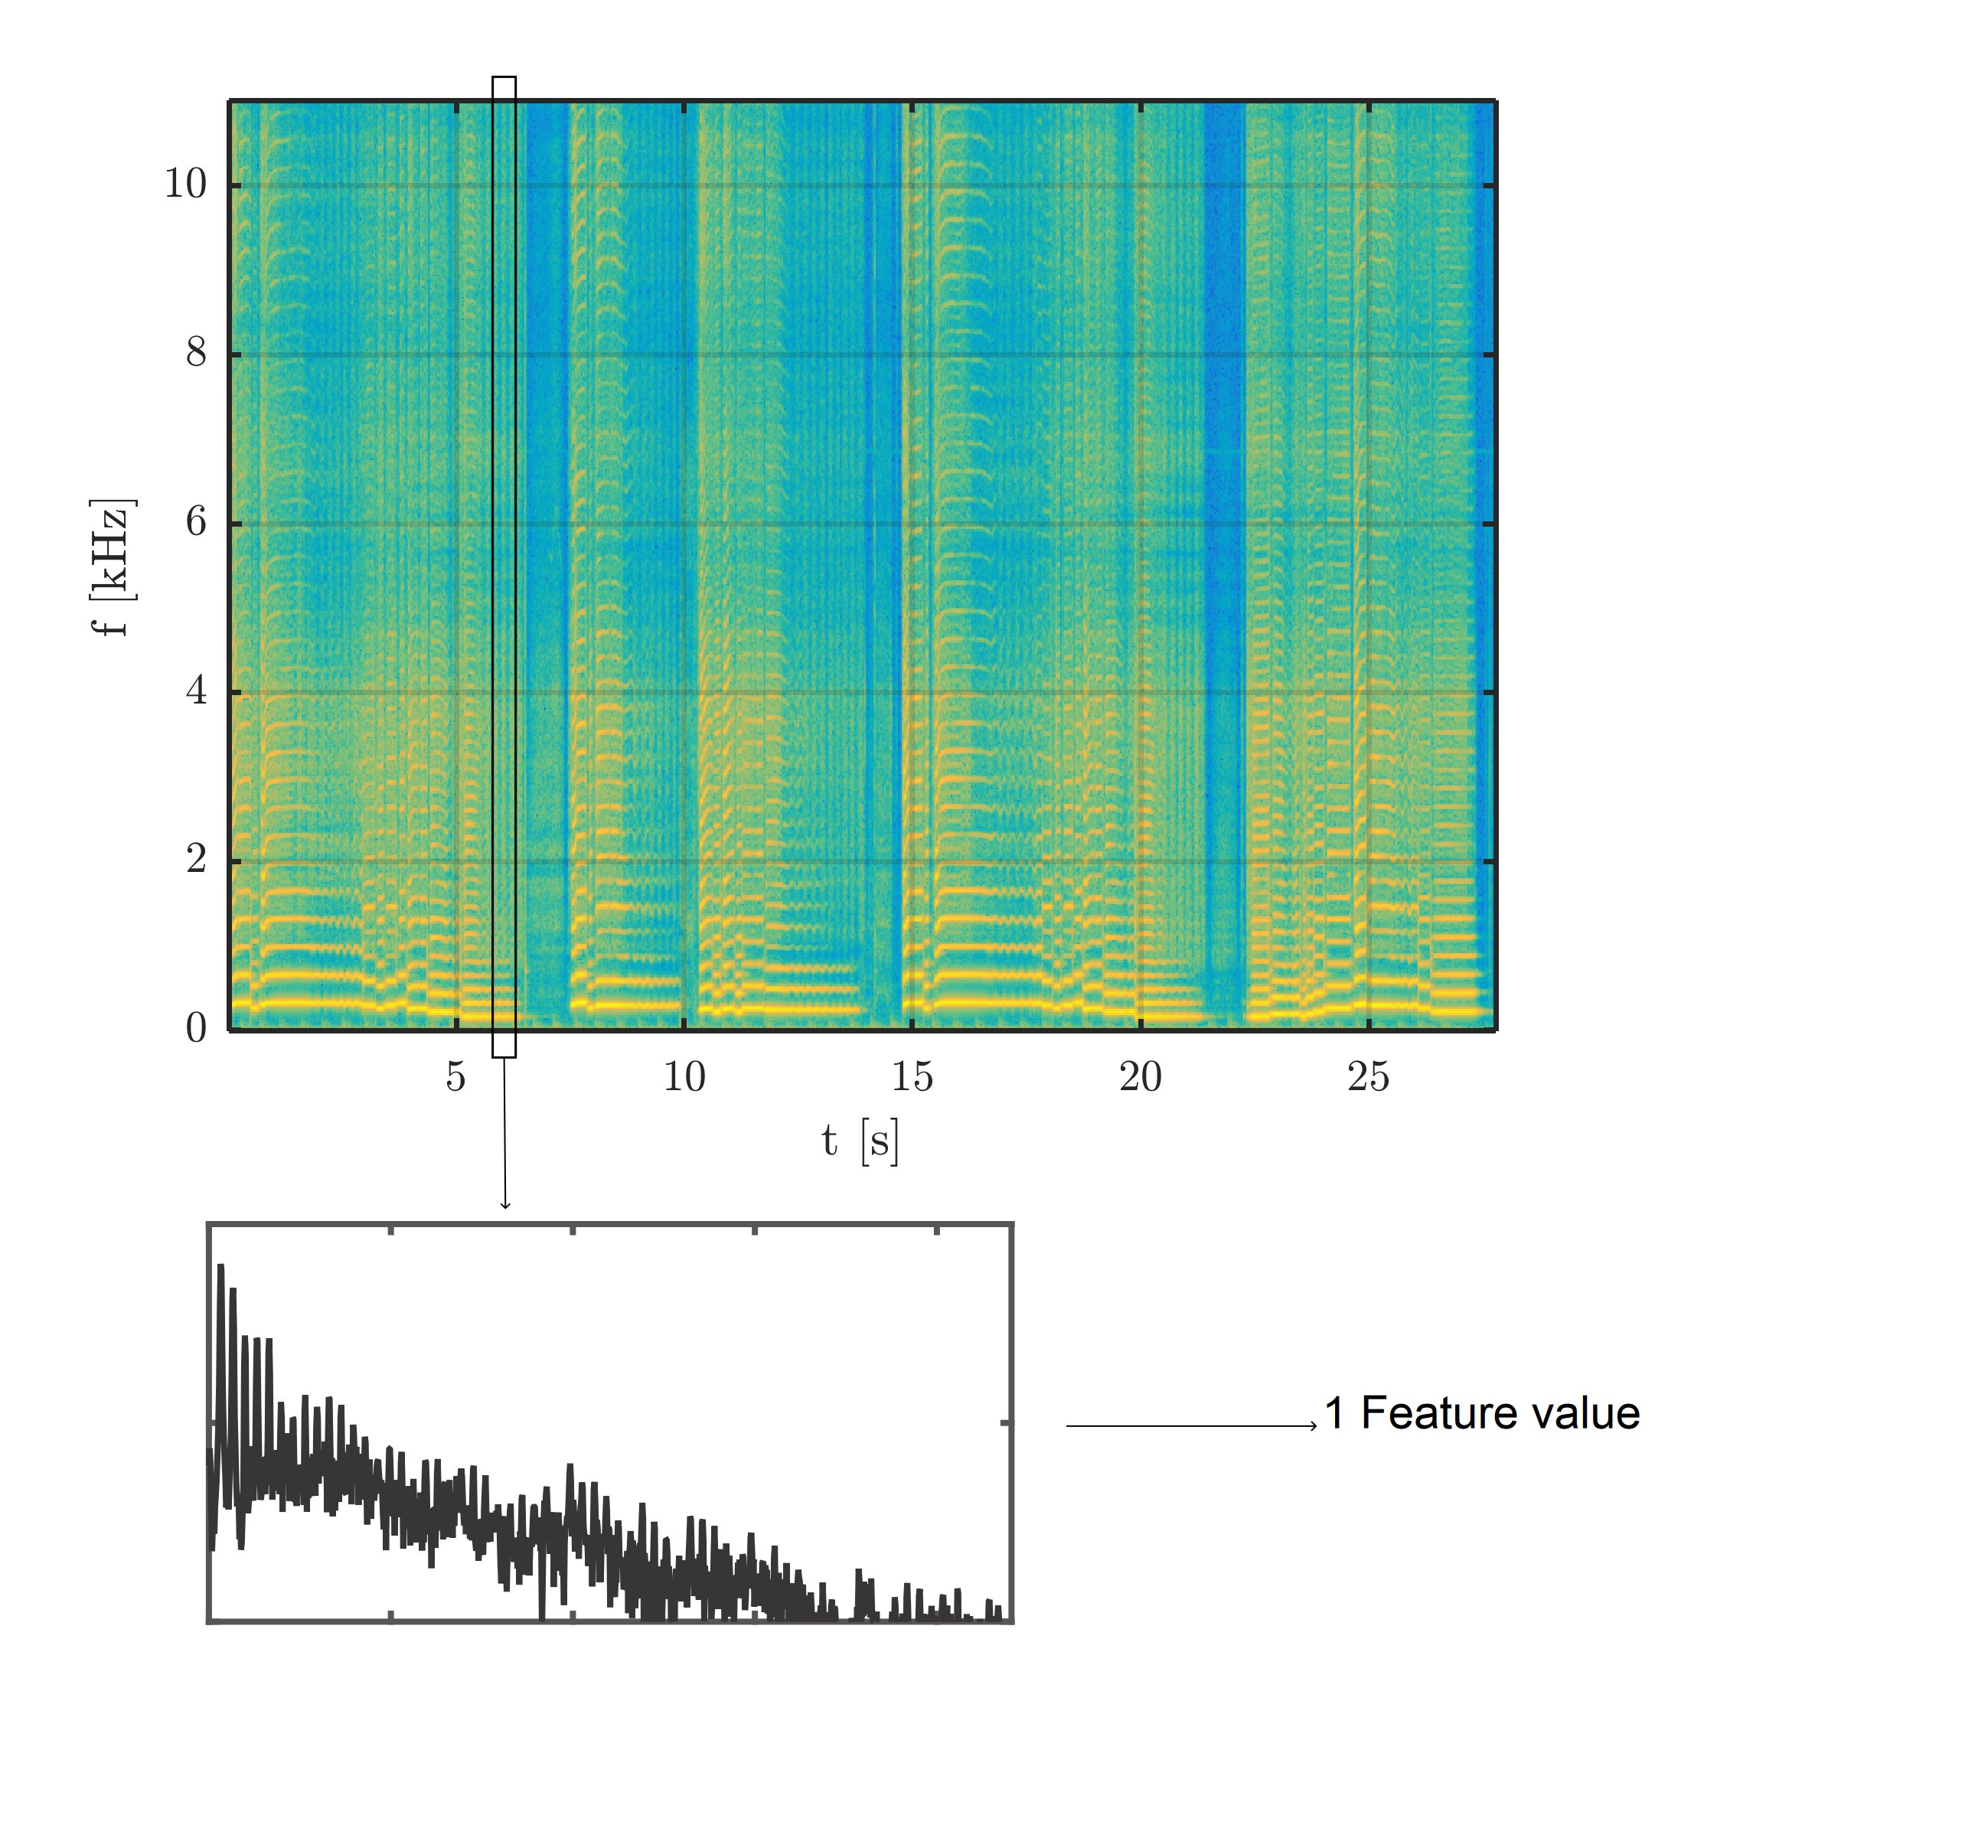
\includegraphics[scale=.08]{FeatureExtraction}
                \end{figure}
                \column{.3\linewidth}
                    \begin{itemize}
                        \item   repeat for every block
                        \item   repeat for every feature
                        \bigskip
                        \item[$\Rightarrow$] feature matrix per audio input
                    \end{itemize}
                \end{columns}
            }
        \end{frame}
        \begin{frame}{instantaneous features}{feature example}
            waveform envelope of three different signals 
            
            \figwithmatlab{Waveforms}
            
            \vspace{-2mm}
            \begin{columns}
                \column{.16\textwidth}
                \column{.25\textwidth}\centering
                    \includeaudio{excerpt_pop}
                \column{.25\textwidth}\centering
                    \includeaudio{excerpt_stringquartet}
                \column{.25\textwidth}\centering
                    \includeaudio{excerpt_speech}
                \column{.09\textwidth}
            \end{columns}
            
            \bigskip
            \begin{itemize}
                \item<2->   envelopes of waveforms can have distinct shape
                \item<3->[$\Rightarrow$] a feature describing the envelope shape should help to distinguish these signal types
            \end{itemize}
        \end{frame}

    \section[pre-proc]{audio pre-processing}
        \begin{frame}{instantaneous features}{audio pre-processing}
            \begin{itemize}
                \item   \textbf{goals} (task dependent)
                    \begin{itemize}
                        \item   reduce amount of data (e.g., down-sampling)
                        \item   remove irrelevant information (e.g., surround channels of multi-channel signal)
                        \item   remove information that might impact analysis (e.g., DC offset)
                        \item   increase robustness (e.g., normalization)
                    \end{itemize}
                 %\bigskip
                %\item<2->   \textbf{examples}
                    %\begin{itemize}
                        %\item   downmix to mono
                        %\item   sample rate reduction
                        %\item   filtering (DC removal, HP, BP, ...)
                    %\end{itemize}
            \end{itemize}
        \end{frame}
        \begin{frame}{instantaneous features}{audio pre-processing examples 1/2}
            \begin{itemize}
                \item   \textbf{down-mixing}
                    \[
                        x(i) = \frac{1}{\mathcal{C}}\sum\limits_{c=0}^{\mathcal{C}-1}{x_c(i)} 
                    \]
                    \begin{itemize}
                        \item   \textit{variants}: different channel weights, $\nicefrac{\pi}{2}$ phase shift in one channel, \ldots
                    \end{itemize}
                    
                \bigskip
                \item<2->   \textbf{normalization}
                    \[
                        x(i) = \frac{x_s(i)}{\max\limits_{\forall i}\big(|x_s(i)|\big)} 
                    \]
                    \begin{itemize}
                        \item   \textit{variants}: RMS, LUFS normalization
                        \item<3>   real-time?
                    \end{itemize}
            \end{itemize}
        \end{frame}
        \begin{frame}{instantaneous features}{audio pre-processing examples 2/2}
            \begin{itemize}
                \item   \textbf{filtering}
                    \begin{itemize}
                        \item   \textit{DC removal}
                            \[
                                x(i) = x_{\mathrm{DC}}(i) - \frac{1}{\mathcal{I}}\sum\limits_{i=0}^{\mathcal{I}-1}{x_{\mathrm{DC}}(i)} 
                            \]
                            \begin{itemize}
                                \item   real-time?
                            \end{itemize}
                        \item   other filters: high/band pass, smoothing, ...
                    \end{itemize}
                \bigskip
                \item<2->   \textbf{sample rate reduction}
                \bigskip
                \item<3->   \textbf{quality enhancement} (denoising etc.)
                \bigskip
                \item<3->   \ldots
            \end{itemize}
        \end{frame}

    \section[stats]{statistical features}
        \begin{frame}{instantaneous features}{statistical features~---~mean 1/3}
			\begin{itemize}
				\item	\textbf{arithmetic mean}
                    \begin{itemize}
						\item   from signal block:
                        
                        \begin{equation*}\label{eq:arith_mean}
							\mu_x(n) = \frac{1}{\mathcal{K}}\sum\limits_{i=i_{\mathrm{s}}(n)}^{i_{\mathrm{e}}(n)}{x(i)} 
						\end{equation*}
                        \pause
                        \item   from distribution:
                        \begin{equation*}\label{eq:arith_mean2}
							\mu_x(n) = \sum\limits_{x=-\infty}^{\infty}{x\cdot p_x(x)} 
						\end{equation*}
                        \pause
                        \item   from unnormalized distribution $d_x$:
                        \begin{equation*}\label{eq:arith_mean3}
							\mu_x(n) = \frac{\sum\limits_{x=-\infty}^{\infty}{x\cdot d_x(x)}}{\sum\limits_{x=-\infty}^{\infty}{d_x(x)}} 
						\end{equation*}
                    \end{itemize}
            \end{itemize}
        \end{frame}
        \begin{frame}{instantaneous features}{statistical features~---~mean 2/3}
			\begin{itemize}
				\item	\textbf{geometric mean}
				\begin{eqnarray*}
					M_x(0,n)		&=& \sqrt[\mathcal{K}]{\prod\limits_{i=i_{\mathrm{s}}(n)}^{i_{\mathrm{e}}(n)}{x(i)}}\label{eq:geo_mean1}\\
								&=& \exp\left({\frac{1}{\mathcal{K}}\sum\limits_{i=i_{\mathrm{s}}(n)}^{i_{\mathrm{e}}(n)}{\log\big[x(i)\big]}}\right) \label{eq:geo_mean2}
				\end{eqnarray*}
                \pause
				\item	\textbf{harmonic mean}
				\begin{equation*}
					M_x(-1,n) = \frac{\mathcal{K}}{\sum\limits_{i=i_{\mathrm{s}}(n)}^{i_{\mathrm{e}}(n)}{\nicefrac{1}{x(i)}}} 
				\end{equation*}
			\end{itemize}
        \end{frame}
        \begin{frame}{instantaneous features}{statistical features~---~mean 3/3}
			\begin{itemize}
				\item	\textbf{generalized mean}
                    \begin{equation*}
                        M_x(\beta,n) = \sqrt[\beta]{\frac{1}{\mathcal{K}}\sum\limits_{i=i_{\mathrm{s}}(n)}^{i_{\mathrm{e}}(n)}{x^\beta(i)}} 
                    \end{equation*}
				\pause
                    \begin{footnotesize}
                    \begin{itemize}
                        \item	{$\beta=1$:} {arithmetic mean}
                        \item	{$\beta=2$:} {quadratic mean}
                        \item	{$\beta=-1$:} {harmonic mean}
                        \item	{$\beta\rightarrow 0$:} {geometric mean}
                        \item	{$\beta\rightarrow -\infty$:} {minimum}
                        \item	{$\beta\rightarrow \infty$:} {maximum}
                    \end{itemize}
                    \end{footnotesize}
			\end{itemize}
        \end{frame}
        \begin{frame}{instantaneous features}{statistical features~---~variance \& standard deviation}
			measure of \textit{spread} of the signal around its mean
            
            \begin{itemize}
                \item \textbf{variance}
                    \begin{itemize}
                        \item   from signal block:
                            \begin{equation*}
                                \sigma_x^2(n) = \frac{1}{\mathcal{K}}\sum\limits_{i= i_{\mathrm{s}}(n)}^{i_{\mathrm{e}}(n)}{\big(x(i)-\mu_x(n)\big)^2} 
                            \end{equation*}
                        \pause
                        \item   from distribution:
                            \begin{equation*}
                                \sigma_x^2(n) = \sum\limits_{x=-\infty}^{\infty}{\big(x-\mu_x\big)^2\cdot p_x(x)} 
                            \end{equation*}
                    \end{itemize}
                \pause
                \item \textbf{standard deviation}
                    \begin{equation*}
                        \sigma_x(n) = \sqrt{\sigma_x^2(n)} 
                    \end{equation*}
            \end{itemize}
        \end{frame}
        \begin{frame}{instantaneous features}{statistical features~---~skewness \& kurtosis}
            \begin{itemize}
                \item \textbf{skewness}: measure of \textit{PDF asymmetry}
                    \begin{equation*}
                        v_{\mathrm{Sk}}(n) = {\frac{1}{\sigma_x^3(n)\cdot \mathcal{K}}\sum\limits_{i=i_{\mathrm{s}}(n)}^{i_{\mathrm{e}}(n)}{\left(\vphantom{\frac{1}{1}}x(i)-\mu_x(n)\right)^3}} 
                    \end{equation*}
                    \begin{footnotesize}
                            \begin{itemize}
                                \item<2->	symmetric PDFs $\rightarrow$ $0$
                                \item<2->	left-skewed (mass center right) $\rightarrow$ negative
                                \item<2->	right-skewed (mass center left) $\rightarrow$ positive 
                            \end{itemize}
                    \end{footnotesize}
                \item<3-> \textbf{kurtosis}: measure of PDF ``\textit{Gaussianity}''
                    \begin{equation*}
                        v_{K}(n) = {\frac{1}{\sigma_x^4(n)\cdot \mathcal{K}}\sum\limits_{i=i_{\mathrm{s}}(n)}^{i_{\mathrm{e}}(n)}{\left(\vphantom{\frac{1}{1}}x(i)-\mu_x(n)\right)^4}} - 3 
                    \end{equation*}
                    \begin{footnotesize}
                            \begin{itemize}
                                \item<4->	Gaussian PDFs (\textit{mesokurtic})  $\rightarrow$ 0
                                \item<4->	flat PDFs (\textit{platykurtic}) $\rightarrow$ negative
                                \item<4->	peaky PDFs (\textit{leptokurtic})  $\rightarrow$ positive
                            \end{itemize}	
                    \end{footnotesize}
            \end{itemize}
        \end{frame}
        \begin{frame}{instantaneous features}{statistical features~---~centroid}
			\setbeamercovered{invisible}
            \textbf{centroid}: \textit{center of gravity}
			\begin{equation*}\label{eq:centroid}
				v_{\mathrm{C}}(n) = \frac{\sum\limits_{i=i_{\mathrm{s}}(n)}^{i_{\mathrm{e}}(n)}{\big(i-i_{\mathrm{s}}(n)\big)\cdot x(i)}}{\sum\limits_{i=i_{\mathrm{s}}(n)}^{i_{\mathrm{e}}(n)}{x(i)}} 
			\end{equation*}
            
            \pause
            \question{Why does this look familiar?}
            
            $\rightarrow$ compare arithmetic mean
        \end{frame}
		\begin{frame}{instantaneous features}{statistical features~---~quantiles \& quantile ranges}
			dividing the PDF into (equal sized) subsets
            \begin{footnotesize}
			\begin{eqnarray*}
				Q_\mathrm{X}(c_p) &=& \argmin\big (F_\mathrm{X}(x) \leq c_p\big)\\
                with\quad F_\mathrm{X}(x) &=& {\int\limits_{-\infty}^{x}{p_\mathrm{x}(y)\, dy}}
			\end{eqnarray*}
            \end{footnotesize}
			\figwithmatlab{PdfQuantiles}
        \end{frame}
		\begin{frame}{instantaneous features}{statistical features~---~quantile examples}
			\begin{itemize}
				\item	\textbf{median}
						\pause
						\begin{equation*}\label{eq:median}
							Q_\mathrm{X}(0.5) = \argmin\big (F_\mathrm{X}(x) \leq 0.5\big)
						\end{equation*}
				\bigskip
				\item<2->	\textbf{quartiles}: $Q_\mathrm{X}(0.25),\, Q_\mathrm{X}(0.5)$, and $Q_\mathrm{X}x(0.75)$
				\bigskip
                \item<3->	\textbf{quantile range}, e.g.
						\begin{equation*}
							\Delta Q_\mathrm{X}(0.9) = Q_\mathrm{X}(0.95)-Q_\mathrm{X}(0.05)
						\end{equation*}
			\end{itemize}
        \end{frame}
		\begin{frame}{instantaneous features}{statistical features~---~matlab exercise}
            \matlabexercise{statistical feature implementation}
            \begin{enumerate}
                \item   load an audio file
                \item   make both block size and hop size parameters of your matlab function
                \item   implement the following features extracted per block of your time domain signal:
                    \begin{itemize}
                        \item   mean and median
                        \item   variance and standard deviation
                        \item   skewness and kurtosis
                    \end{itemize}
            \end{enumerate}
		\end{frame}

    \section[summary]{lecture summary}
        \begin{frame}{summary}{lecture content}
            \begin{enumerate}
                \item       what is a low level feature? 
                \smallskip
                \item<2->   name examples of low level features
                \smallskip
                \item<3->   name typical pre-processing steps and use cases for which these steps are beneficial
                \smallskip
                \item<4->   name features describing the PDF of a signal and discuss possible benefits and disadvantages of those features
                \smallskip
                \item<5->   what are commonalities of the equations of the measures variance, skewness, and kurtosis
            \end{enumerate}
        \end{frame}
\end{document}

